\documentclass{article}
\usepackage[UKenglish]{babel}
% \usepackage{fontspec}
% \usepackage{polyglossia}
% \usepackage{unicode-math}
\usepackage{minted}
% \usepackage[mathletters]{ucs}
\usepackage[utf8]{inputenc}
\usepackage{listings}
\usepackage{xcolor}
\usepackage{quiver}
\usepackage[pdf]{graphviz}
\usepackage{caption, subcaption}
\usepackage[toc,page]{appendix}
\usepackage{bbm}
\usepackage{dsfont}
\usepackage{lastpage}
\usepackage{fancyhdr}
\pagestyle{fancy}
\fancyhf{}
\renewcommand{\headrulewidth}{0pt}

\cfoot{\thepage\ / \pageref{LastPage}}

\definecolor{codegreen}{rgb}{0,0.6,0}
\definecolor{codegray}{rgb}{0.5,0.5,0.5}
\definecolor{codepurple}{rgb}{0.58,0,0.82}
\definecolor{backcolour}{rgb}{0.95,0.95,0.92}
\lstdefinestyle{mystyle}{
    backgroundcolor=\color{backcolour},
    commentstyle=\color{codegreen},
    keywordstyle=\color{magenta},
    numberstyle=\tiny\color{codegray},
    stringstyle=\color{codepurple},
    basicstyle=\ttfamily\footnotesize,
    breakatwhitespace=false,
    breaklines=true,
    captionpos=b,
    keepspaces=true,
    numbers=left,
    numbersep=5pt,
    showspaces=false,
    showstringspaces=false,
    showtabs=false,
    tabsize=2
}

\lstset{style=mystyle}

\usepackage{tabularx}
\usepackage{booktabs}
\renewcommand{\arraystretch}{1.5}

\usepackage{mathtools}
\setcounter{MaxMatrixCols}{20}
\usepackage{enumitem}
\setenumerate[0]{label=(\arabic*)}

\usepackage[linesnumbered,ruled,vlined]{algorithm2e}
\newcommand\mycommfont[1]{\footnotesize\ttfamily\textcolor{blue}{#1}}
\SetCommentSty{mycommfont}

\SetKwInput{KwInput}{Input}                % Set the Input
\SetKwInput{KwOutput}{Output}              % set the Output


% Kan Danny godt lide!
\usepackage[autostyle]{csquotes}
\usepackage{kpfonts}
\usepackage{inconsolata}
\linespread{1.06}

\usepackage{xcolor}
\usepackage{xurl}
\usepackage{hyperref}
\hypersetup{%
	pdftitle=Reinforcement learning for mathematical applications,
	pdfauthor={Andreas Bøgh Poulsen},
	colorlinks,
	linkcolor={red!50!black},
	citecolor={red!50!black},
	urlcolor={red!50!black},
	bookmarksnumbered=true
}

\usepackage[ntheorem]{mdframed}
\usepackage[amsmath,thmmarks,hyperref]{ntheorem}
\usepackage[capitalize]{cleveref}

% Frame for theorems
\definecolor{shadecolor}{gray}{0.93}
\definecolor{rulecolor}{gray}{0.4}
\mdfdefinestyle{thmframed}{%
	%usetwoside=false, % For use with memoir twoside
	skipabove=0.5em plus 0.4em minus 0.2em,
	skipbelow=0.5em plus 0.4em minus 0.2em,
	leftmargin=-7pt, rightmargin=-7pt, innerleftmargin=6pt,
	innerrightmargin=6pt, innertopmargin=6pt, innerbottommargin=3pt,
	linewidth=1pt, linecolor=rulecolor, backgroundcolor=shadecolor,
	splittopskip=1.2em minus 0.2em,
	splitbottomskip=0.5em plus 0.2em minus 0.1em,
}

% New theorem style with a dot
\makeatletter
\newtheoremstyle{changedot}%
  {\item[\hskip\labelsep \theorem@headerfont ##2~~$\cdot$~~##1\theorem@separator]}%
  {\item[\hskip\labelsep \theorem@headerfont ##2~~$\cdot$~~##1\ (##3)\theorem@separator]}

\newtheoremstyle{changedotbreak}%
  {\item\hbox to \textwidth{\theorem@headerfont ##2~~$\cdot$~~##1\theorem@separator\hfill}}%
  {\item\hbox to \textwidth{\theorem@headerfont ##2~~$\cdot$~~##1\
      (##3)\theorem@separator\hfill}}
\makeatother

\theoremstyle{changedot}
\theoremseparator{.}
\newmdtheoremenv[style=thmframed]{theorem}{Theorem}[section]
\newmdtheoremenv[style=thmframed]{proposition}[theorem]{Proposition}
\newmdtheoremenv[style=thmframed]{lemma}[theorem]{Lemma}
\newmdtheoremenv[style=thmframed]{corollary}[theorem]{Corollary}

\theorembodyfont{\normalfont}
%\theoremsymbol{\ensuremath{\triangle}}
\newmdtheoremenv[style=thmframed]{definition}[theorem]{Definition}

\theoremstyle{changedotbreak}
\newmdtheoremenv[style=thmframed]{definitionbreak}[theorem]{Definition}

\theoremstyle{nonumberplain}
\theoremheaderfont{\normalfont\itshape}
\theorembodyfont{\normalfont}
\theoremsymbol{\ensuremath{\square}}
\newtheorem{proof}{Proof}
\newtheorem{remark}{Remark}
\newtheorem{example}{Example}

\Crefname{theorem}{Theorem}{Theorems}
\Crefname{proposition}{Proposition}{Propositions}
\Crefname{lemma}{Lemma}{Lemmata}
\Crefname{corollary}{Corollary}{Corollaries}
\Crefname{definition}{Definition}{Definitions}

\crefformat{equation}{(#2#1#3)}

% / Kan Danny godt lide

% Kan Andreas godt lide
\setlength{\parindent}{1em}
\setlength{\parskip}{0.7em}


\title{Reinforcement learning for mathematical applications}
\author{
    Andreas Bøgh Poulsen\\
    201805425
}
% \date{28th June 2020}


\usepackage{csquotes}
\usepackage[backend=biber, style=alphabetic, maxcitenames=1]{biblatex}
\addbibresource{references.bib}

\usepackage{microtype}

\usepackage{graphicx}




\newcommand{\ro}[1]{^{\setminus #1}}
\newcommand{\rr}  {^{\setminus}}

\DeclarePairedDelimiter{\tuple}{\langle}{\rangle}
\newcommand{\calM}{\mathcal{M}}
\newcommand{\calV}{\mathcal{V}}
\newcommand{\calD}{\mathcal{D}}
\newcommand{\calG}{\mathcal{G}}

\newcommand{\m}{\mathbb}

\newcommand{\true}{\textsc{true}}
\newcommand{\false}{\textsc{false}}

\DeclareMathOperator{\lcm}{lcm}

\DeclareMathOperator*{\smallbigcup}{\textstyle\bigcup}
\DeclareMathOperator*{\bigunion}{\mathchoice
	{\smallbigcup}%
	{\bigcup}%
	{\bigcup}%
	{\bigcup}%
}
\DeclareMathOperator*{\smallbigcap}{\textstyle\bigcap}
\DeclareMathOperator*{\bigintersect}{\mathchoice
	{\smallbigcap}%
	{\bigcup}%
	{\bigcup}%
	{\bigcup}%
}

\DeclarePairedDelimiter{\abs}{\lvert}{\rvert}
\DeclarePairedDelimiter{\norm}{\lVert}{\rVert}

\newcommand{\setN}{\mathbb{N}}
\newcommand{\setR}{\mathbb{R}}
\newcommand{\card}[1]{\abs{#1}}

\let\phi\varphi
\frenchspacing

% Partial functions
% From https://tex.stackexchange.com/questions/47142/how-to-tex-an-arrow-with-vertical-stroke

\makeatletter
\newcommand{\pto}{}% just for safety
\newcommand{\pgets}{}% just for safety

\DeclareRobustCommand{\pto}{\mathrel{\mathpalette\p@to@gets\to}}
\DeclareRobustCommand{\pgets}{\mathrel{\mathpalette\p@to@gets\gets}}

\newcommand{\p@to@gets}[2]{%
  \ooalign{\hidewidth$\m@th#1\mapstochar\mkern5mu$\hidewidth\cr$\m@th#1\to$\cr}%
}
\makeatother

\newcommand{\id}{\mathrm{id}}
\DeclarePairedDelimiter{\ceil}{\lceil}{\rceil}
\DeclarePairedDelimiter{\floor}{\lfloor}{\rfloor}
\DeclarePairedDelimiter{\anglemap}{\langle}{\rangle_{\infty}}

\newcommand{\nextk}{\mathrm{next}}
\newcommand{\enc}{\mathrm{enc}}

\newcommand{\binlit}[1]{\mathbf{#1}}
\newcommand{\bin}{\mathrm{bin}}
\newcommand{\val}{\mathrm{val}}
\newcommand{\Seq}{\mathrm{Seq}}
\newcommand{\length}[1]{\abs{#1}}

\DeclarePairedDelimiter{\gpath}{\langle}{\rangle}

% \newcommand{Hrule}{\hrule width \hsize \kern 1mm \hrule width \hsize height 2pt}

\begin{document}

\begin{titlepage}
  \center \sc
  % \noindent\Hrule{}
  \hrule width \hsize height 2pt \kern 1mm \hrule width \hsize
  \vspace{4mm}
  \noindent{\Large Reinforcement learning \\ with an application to Gröbner bases}
  \vspace{6mm}
  \hrule width \hsize \kern 1mm \hrule width \hsize height 2pt
  \vspace{10mm}
  \noindent{\large Bachelor's project in Mathematics \\ July 10, 2021}

  \vspace{10mm}

  \includegraphics[width=0.7\textwidth]{au_gammel.png}

  \vspace{15mm}

  {\large Andreas Bøgh Poulsen, student number: 201805425 \\ Supervisor: Niels Lauritzen}

  \vspace{7mm}

  \includegraphics[width=0.4\textwidth]{aulogo_uk_var2_blue.png}
\end{titlepage}

\begin{abstract}
  Dylan Peifer et al \cite{peifer} showed the potential of using machine learning techniques in pure mathematics by having a neural network improve the performance of Buchberger's algorithm, used to compute Gröbner bases. Not only that, but they developed a new selection strategy by interpreting the actions of the network, which also improves performance over existing strategies. They also introduced this as a challenge for other researchers to improve their results.

  This project have written an environment in Julia to train and evaluate neural networks, similar to the python code Peifer et al used for their article, and attempted two simpler techniques: policy gradient without Generalized Advantage Estimation and Q-learning. Using policy gradients without GAE we obtain performance similar to existing strategies but lower than Peifer et al, and with Q-learning we obtain worse performance but better than random. This indicates that reducing variance in rewards is the way to make progress on this problem.

  This rapport is intended for two audiences: first for people who read \cite{peifer} and wish for some more background and second as an example for mathematicians who want to introduce machine learning in their own research.
\end{abstract}

\newpage

\tableofcontents

\newpage

\section{Introduction}
In 2020 Dylan Peifer et al \cite{peifer} showed how to use deep learning to improve the performance of algorithms for constructing Gröbner bases. The goal of this project was to reproduce the results of this paper using their method of policy gradient learning as well as attempt to use a simpler technique called Q-learning.

Gröbner bases have many applications for example in integer programming (solving or optimizing equations of intergers), but for reasons we will discuss later, only binomial ideals i.e. ideals of polynomials with at most two terms, will be considered. These still have many applications, for example in considerations using \emph{lattice ideals} which are generated by binomials in which each variable appears in only one of the terms. These have applications in optimization and integer programming, for example \cite{lattice} or in computing Frobenius numbers \cite{frobenius}.

This project have almost reproduced the results of \cite{peifer}. We have written a complete code package to work with multinomials and compute Gröbner bases and using this code we have trained two neural networks on the same problem as \cite{peifer}, one using a simpler version of their technique called policy gradients and another using a more classical approach called Q-learning. 

The structure of this report is as follows: first, we'll briefly cover Gröbner bases, their uses and how to compute them. Next, the use of reinforcement learning, a branch of deep learning used by Peifer et al. We'll cover both the conceptual framework, as well as two particular techniques: Q-learning and policy gradients. The third part covers our experimental results featuring both an evaluation of existing heuristics as well as our results. Last is a walk-through of the code produced during this project, how to use it and how it's structured.

\section{Gröbner bases}

Since the problem we're considering is the construction of Gröbner bases, let's give a short introduction to Gröbner bases.

We fix a field $k$ and consider the polynomial ring $R = k[x_{1}, \dots, x_{n}]$. For a set of polynomials $F = \{f_{1}, \dots, f_{l}\}$ we consider the ideal $I = \tuple{f_{1}, \dots, f_{l}}$ generated by these polynomials. Now, we wish to efficiently determine whether a given polynomial $f$ lies in $I$ or not. The standard way to prove that $R$ is a \emph{unique factorization domain} gives a division algorithm which can be used to decide whether $f \in I$ or not, but giving an efficient algorithm is tricky. Instead, we can extend the generating set of the ideal in a way that doesn't change the ideal but gives us stronger properties, enabling an efficient decision algorithm.

Fix a \emph{term order} which is a well-order relation $>$ on $\mathbb N^{n}$ such that $a > b$ implies $a + c > b + c$ for any $a, b, c \in \mathbb N^{n}$. This naturally extends to a so called \emph{monomial order} on monomials $\{x^{v} = x_{1}^{v_{1}} \cdots x_{n}^{v_{n}} \mid v \in \mathbb N^{n}\}$ by comparing exponent vectors of the monomials. We'll write $>$ for both orders.

There are two common term orders: lexicographic and grevlex. Lexicographic has $a > b$ if there exists $k$ s.t. $a_{i} = b_{i}$ for $i < k$ and $a_{k} > b_{k}$. This is the usual ``alphabetic order'' on tuples. Grevlex ordering is often used in implementations using Gröbner bases and has $a > b$ if $\sum_{i} a_{i} > \sum_{j} b_{j}$ or   $\sum_{i} a_{i} = \sum_{j} b_{j}$ and the last non-zero entry of $a - b$ is negative. In two dimensions, this means $a > b$ if the 1-norm of $a$ is greater than that of $b$ or, if they're equal, that a is further up a top-left-to-bottom-right diagonal than $b$. In the following example, given $a=(1, 3)$, $b=(3, 1)$ and $c=(1, 1)$, we have that $a > b > c$:

\begin{center}
  \includegraphics[width=0.5\textwidth]{desmos-graph.png}
\end{center}

Proving that these are monomial orders is left af an excercise to the reader. Grevlex order is often used in implementations of Gröbner bases and that is what we use onwards.

Given a monomial order, we can define the \emph{initial term} and the S-polynomial.

\begin{definition}
  Given a monomial order $>$, the \emph{initial term} or \emph{leading term} of a polynomial $f = \sum_{v} \lambda_{v} x^{v}$, denoted $in_{>}(f)$ is the greatest term of $f$ with respect to $>$. We will often omit the subscript when the order is either clear from context or arbitrary.
\end{definition}

Recall that the division algorithm for polynomials of a single variable considers whether the leading term of the dividend is divisible by the leading term of any of the divisors and subtracts a proper multiple of that divisor if it is. Using monomial orders, this algorithm translates directly to multinomials:

\begin{algorithm}[H]
\DontPrintSemicolon

  \KwInput{Polynomial $f$ and $F = \{f_{1}, \dots, f_{l}\}$}
  \KwOutput{Remainder $r$ s.t. $f - r \in \tuple F$ and $in(f_{i}) \nmid in(r)$ for all $f_{i} \in F$}
  $r \leftarrow f$\;
  \While{$\exists i. in(f_{i}) \mid in(r)$}
    {
        $r \leftarrow r - \frac{in(r)}{in(f_{i})} f_{i}$
    }

    \caption{Division algorithm $reduce(f, F)$}
    \label{alg:div}
\end{algorithm}

This algorithm terminates since the initial term of $r$ is strictly decreasing with respect to $>$. However, this algorithm has some problems. In particular, we do not always get that $\text{reduce}(f, F) = 0$ when $f$ lies in the ideal generated by $F$, as we would expect. For example if $F = \{xy+x, xy+y\}$ and $I = \tuple{F}$ then $f = (xy+x) - (xy+y) = x+y \in I$ but $\text{reduce}(f, F) = x+y$ since no initial term divides $x$ or $y$. For a less trivial example, see 5.4.3 in \cite{NL}.

Now, we're ready to present Gröbner bases and the theorem that makes them so important:

\begin{definition}
  A Gröbner basis for an ideal $I$ is a set of polynomials $F = \{f_{1}, \dots, f_{l}\} \subseteq I$ such that $in(f_{i}) \mid in(f)$ for all $f \in I\setminus \{0\}$.
\end{definition}
Note that this definition implies $\tuple F = I$.

\begin{theorem}
  Let $G = \{f_{1}, \dots, f_{l}\}$ be a Gröbner basis for the ideal $I = \tuple{G}$. Then $reduce(f, G) = 0 \Longleftrightarrow f \in I$.
\end{theorem}
\begin{proof}
  If $reduce(f, G) = 0$ then $f = f - 0 \in I$.

  If $f \in I$ and $f - r = h \in I$ then $r = f - h \in I$. But as guaranteed by the division algorithm, there is no $f_{i} \in G$ where $in(f_{i}) \mid in(r)$ even though $G$ is a Gröbner basis. The only element in $I$ not subject to the Gröbner basis constraint is zero, thus $r$ must be zero.
\end{proof}

So, Gröbner bases are great, but how do we construct them? Do they even exist for every ideal? They do exist and we have an algorithm called Buchberger's algorithm to find them, but first, we need a construction called the S-polynomial or syzygy polynomial.

\begin{definition}
  The S-polynomial or syzygy polynomial of two polynomials $f$ and $g$ is denoted $S(f, g) = \frac{x^{w}}{in(f)} f - \frac{x^{w}}{in(g)} g$ where $x^{w} = \lcm(in(f), in(g))$ is a least common multiple of the leading terms of $f$ and $g$.
\end{definition}

The Buchberger criterion is a simple way to check if we have a Gröbner basis, and it even leads us to an algorithm for constructing Gröbner bases.

\begin{theorem}[Buchberger's criterion]\label{thm:buchberger_crit}
Let $F = \{f_{1}, \dots, f_{l}\}$ be a set of polynomials and let $I = \tuple F$ be the ideal generated by $F$. If $\text{reduce}(S(f_{i}, f_{j}), F) = 0$ for all $f_{i}, f_{j} \in F$ then $F$ is a Gröbner basis for $I$.
\end{theorem}

The idea behind Buchberger's algorithm is very simple: We simply see if Buchberger's criterion holds. If it does, we're done. If it doesn't, there is some S-polynomial that doesn't reduce to 0. Add the remainder of that S-polynomial to the basis and try again. When the algorithm terminates (proof of termination is theorem 5.7.2 in \cite{NL}) every S-polynomial will reduce to 0, so by theorem \ref{thm:buchberger_crit} we have a Gröbner basis. In pseudo-code the algorithm is:

\begin{algorithm}[H]
  
\DontPrintSemicolon

  \KwInput{A set of polynomials $F = \{f_{1}, \dots, f_{l}\}$}
  \KwOutput{A Gröbner basis $G$ of the ideal $I = \tuple F$}
  $G \leftarrow F$ \;
  $P \leftarrow \{(f_{i}, f_{j}) \mid 1 \leq i < j \leq l\}$ \;
  \While{$|P| > 0$}
  {
    $(g, h) \leftarrow \text{select}(P)$ \;
    $P \leftarrow P \setminus \{(g, h)\}$ \;
    $r \leftarrow \text{reduce}(S(g, h), G)$ \;
    \If{$r \neq 0$}
    {
      $P \leftarrow \text{update}(P, G, r)$ \;
      $G \leftarrow G \cup \{r\}$ \;
    }
  }

\caption{Buchbergers algorithm}
\end{algorithm}

Notice that the algorithm uses two subroutines we haven't defined: \emph{select} and \emph{update}. The simplest implementations are $\text{select( $P$ )} = P_{1}$ taking the first pair in $P$ and $\text{update( $P, G, r$ )} = P \cup \{(f, r) \mid f \in G\}$. We'll see better and more refined implementations later.

To produce a faster version of Buchberger's algorithm, these two subroutines are good places to start. During \emph{update} we can eliminate a large number of pairs using simpler criteria than theorem \ref{thm:buchberger_crit}. We'll discuss a better version in section \ref{sec:update}.

\subsection{A better \emph{select}} \label{sec:select}

The problem of selecting the next pair of polynomials is not easy and it turns out to have serious consequences. Simply switching from taking the first pair to taking the last one, i.e. treating $P$ as a stack instead of a queue, can reduce the number of polynomial additions by almost 50\% as seen in table \ref{tab:std_perf}. Since the goal of this project is to improve the selection strategy, let's look at some standard selection strategies

\begin{itemize}
  \item[Random] Pick a random pair uniformly.

  \item[First] Pick the lexicographically smallest pair, where the order of polynomials is given by their order in $G$. This is more systematic than picking randomly, and ensures that S-pairs coming from the original generating set is reduced first, which seems to be an advantage.

  \item[Queue] Treat $P$ as a queue and select the pair that was added first. This also ensures that S-pairs coming from the original generating set is reduced first and does so in a slightly more computer-friendly way than \emph{first} since queue is a simple datastructure.

  \item[Stack] Treat $P$ as a stack and select the pair that was most recently added. This strategy is very easy to implement, a stack is one of the simples datastructures, but its performance is horrible. A good example that we can devise worse strategies than picking at random.

  \item[Degree] Pick the pair $(f, g)$ with the smallest total degree of $\lcm(in(f), in(g))$. Polynomials with small degrees have better chances of dividing future polynomials, so it makes sense to add them early on. This is the usual choice of selection strategy.

  \item[Normal] Pick the pair $(f, g)$ where $\lcm(in(f), in(g))$ is smallest in the used monomial order. This is a refinement of \emph{degree} but is very dependent on the choice of monomial order. In grevlex it doesn't outperform \emph{degree}.

  \item[Sugar] Pick the pair $(f, g)$ with the smallest \emph{sugar degree} which is the degree $\lcm(in(f), in(g))$ would have had if the polynomials had been homogenized. Introduced in \cite{sugar} to improve performance on traditionally challenging ideals.

  \item[TrueDegree] Introduced in \cite{peifer}, pick the pair $(f, g)$ whose S-polynomial has the lowest total degree. This strategy is an approximation of what their neural network have learned and outperforms all of the strategies above.
\end{itemize}


\subsection{A better \emph{update}}  \label{sec:update}
In the Buchberger algorithm, a pair $(f, g)$ will be removed if $\text{reduce}(S(f, g), G) = 0$. However, this is a computationally expensive test. Fortunately, there are some easier tests that can eliminate a large number of pairs. I'll describe the tests given by Gebauer \& Möller \cite{GM}. The advantage of using these tests can be seen in table \ref{tab:imp_details}.

\subsubsection{Operational description}
Gebauer \& Möller reduction is performed as part of the procedure $\text{update}(P, G, r)$. First, in the pair set $P$ we remove every pair $(f, g)$ where $in(r) | \lcm(in(f), in(g))$ and $\lcm(in(f), in(r)) \neq \lcm(in(f), in(g)) \neq \lcm(in(g), in(r))$.

Next, consider the set $P' = \{(f, r) \mid f \in G\}$. These are all the pairs we should naively add to $P$. Partition $P'$ into equivalence classes using the equivalence realation $(f, r) \sim (g, r) \Longleftrightarrow \lcm(in(f), in(r)) = \lcm(in(g), in(r))$. Remove every equivalence class containing no element $(f, r)$ satisfying $\lcm(in(f), in(r)) = in(f) in(r)$ and take a representative from each remaining equivalence class. Let $P''$ be this set of representatives and let $P \cup P''$ be the result of $\text{update}(P, G, r)$.


\subsubsection{Justification and proof}
Simply put, Gebaur\& Möller reduction consists of reducing a Gröbner basis. Once a Gröbner basis is constructed, we may throw away any redundant element. This process is described above and the proof that this maintains the Gröbner basis property can be found in \cite{NL} section 5.8.

For the setup we need to extend the concept of Gröbner bases to free modules over a polynomial ring. Let $R$ be a multinomial ring in $n$ variables over a field $k$ and $e_{1}, \dots, e_{m}$ be the canonical basis of $R^{m}$. Since every element of $R^{m}$ is a $k$-linear combination of elements of the form $x^{v}e_{i}$, $v \in \m N^{n}$, we call these $x^{v}e_{i}$ for monomials. Now, the definition of Gröbner bases require two more parts: a monomial order and a divisability test. Monomial orders work the same way, they're a total order satisfying \[x^{v_{1}}e_i < x^{v_{2}}e_{j} \Longrightarrow x^{v_{1} + v} e_{i} < x^{v_{2} + v} e_{j}\] for all $v \in \m N^{n}$. We say that $x^{v_{1}}e_{i}$ divides $x^{v_{2}}e_{j}$ iff $i=j$ and $x^{v_{1}}$ divides $x^{v_{2}}$. Now, the definition of a Gröbner basis is the same, and we will repeat it here: a Gröbner basis for a submodule $M \subset R^{m}$ is a set of elements $F = \{m_{1}, \dots, m_{t}\} \subset M$ such that $in(m_{i})$ divides $in(m)$ for all $m \in M \setminus \{0\}$.

Now, consider the ideal of monomials $I = \tuple{x^{v_{1}}, \dots, x^{v_{m}}} \subset R$ and the natural surjection $p : R^{m} \to I$ sending $e_{i}$ to $x^{v_{i}}$. Now, let $K$ be the kernel of $p$ and notice that the syzygies in $I$ are a basis of $K$.

\begin{example}
If $I = \tuple{x, y, z}$ then $K$ will have a basis consisting of the syzygies $\{x e_{2} - y e_{1}, x e_{3} - z e_{1}, y e_{3} - z e_{2}\}$. 
\end{example}

More generally, the elements \[S_{ij} = x^{\lcm(v_{i}, v_{j}) - v_{j}} e_{j} - x^{\lcm(v_{i}, v_{j}) - v_{i}} e_{i}, \, \, 1 \leq i < j \leq m\] are basis elements of $K$. However, this basis is usually not minimal. Now, we need two propositions, the first due to Schreyer.

\begin{theorem}
 There exists a monomial order called the Schreyer order such that set $\{S_{ij} \mid 1 \leq i < j \leq m\}$ is a Gröbner basis for $K$ over this order.
\end{theorem}

The second is proposition 2.9.9 from \cite{IVA}.

\begin{theorem}
  Let $G = \{g_{1}, \dots, g_{m}\}$ be a generating set for an ideal $I$. Then $G$ is a Gröbner basis for $I$ iff for every basis element of the syzygies of G $S = \sum_{i = 1}^{m} x^{u_{i}} e_{i}$ we have $\sum_{i=1}^{m} x^{u_{i}} g_{i} \to_{G} 0$.
\end{theorem}

Note that $f \to_{G} 0$ in this context simply means reduces to zero using a generalized version of the multivariate division algorithm. In general the concept is more complex, see \cite{IVA} definition 1 of section 2.9.

Now, this is a refinement of the Buchberger S-criterion. It is therefore enough to reduce the S-polynomials corresponding to any Gröbner basis of the syzygies. In particular, we may take the basis $\{S_{ij} \mid 1 \leq i < j \leq m\}$ and reduce it to a minimal Gröbner basis before reducing mod $G$ and adding to $G$.


\section{Abstract framework of deep learning}

We'll use modern advances in machine learning to learn a better selection strategy for Buchberger's algorithm. If you don't know what machine learning is, the next subsection is a quick introduction. We'll need a branch of machine learning called ``reinforcement learning'' which we'll introduce afterwards.

\subsection{Machine learning}
Machine learning is a technique to approximate any function given some sampled inputs and outputs. Classical techniques include linear regression and support vector machines but I'll focus on neural networks as we use those in this project.

A layer of neurons is an affine transformation of the form $\m R^{n} \ni x \mapsto Ax + b$ for some matrix $A$ and vector $b$, followed by a non-linear function called the \emph{activation function} applied to every entry of the resulting vector. Typical choices here are the sigmoid function, tanh or relu, defined as $relu(x) = \mathds{1}_{\left[0,\infty\right)}(x) x$ i.e. constantly zero for negative arguments and the identity for positive arguments. A neural network is then a composition of several layers of neurons.

Now, suppose we have a neural network, denoted by $N$ and we would like this network to approximate a function, say the constant function $\m R \ni x \mapsto 0$. Then we'd sample some values in the domain $x_{1}, x_{2}, \dots \in \m R$ and compute the corresponding function values $y_{1}, y_{2}, \dots = 0, 0, \dots$, called \emph{labels}. Next, compute a \emph{loss} value, which is ``how wrong'' the network was: \[loss = \sum_{i} (y_{i} - N(x_{i}))^{2}.\] Since everything in this expression is differentiable\footnote{Technically, $relu$ is only differentiable almost-everywhere.}, we can get a derivative of this expression and by using an algorithm called \emph{backpropagation} we can propagate this derivative back through the layers. By following the direction of the derivative we can update every parameter in the neural network (each entry in the matrices and vectors) make the loss slightly smaller. Repeating this process will eventually yield a good approximation of the input function.

This technique can be applied to many domains. Recognizing whether a picture contains a bird or not is a function from images to a boolean value. Speech transciption is a function from a waveform to a sequence of words. Playing chess is a function from a board state to an action, repeated many times.

Usually, when machine learning we don't have direct access to the function we're trying to approximate. Instead we collect a dataset, a large number of input/output pairs, and hope they cover enough of the domain for the neural network to learn the right function. Such a dataset could be pictures where humans have identified whether they contain birds or not.

Mathematical applications such as pair selection shine here. It's often expensive to collect a large dataset in the real world but polynomial ideals are very easy to come across (just sample a few polynomials and take the ideal generated by them) and we have a method for finding Gröbner bases already. That means we can generate very large datasets for almost free.

Similarly, A. Z. Wagner\cite{RLgraphs} used machine learning to construct counterexamples to conjectures in graph theory. For example they disprove the conjecture that the sum of a graphs largest eigenvalue $\lambda_{1}$ and it's matching number $\mu$ is greather than $\sqrt{n - 1} + 1$ where $n$ is the number of nodes in the graph, i.e. $\lambda_{1} + \mu \geq \sqrt{n - 1} + 1$. By using $\lambda_{1} + \mu$ as their loss function, their neural network learned to minimize that until it reached below the threshold.

We'll use neural networks to learn a better selection strategy for Buchberger's algorithm. However, we'll need a modification. A normal neural network gives a single output which can then be evaluated. Buchberger's algorithm calls the select function several times and we need to complete the algorithm before we can tell how well we did. We also don't know what the ``correct'' action is, we just know how good a run of the algorithm performed. Reinforcement learning is a family of solutions to these problems. They don't require labels, only a loss function telling us how good a series of predictions were.

\subsection{Reinforcement-learning and Markov Decision Processes}

Constructing Gobner bases can be seen as an interaction between an agent and an environment: we pick a pair to reduce, perform polynomial reduction, add some new pairs to the set of pairs and go again. We want to do the least amount of work when we're done. This interaction can be modeled using Markov decision processes.

A Markov decision process (MDP for short) is an interaction between an environment and an agent. At timestep $t = 0, 1, 2, \dots$ the agent recieves a \emph{state}, $s_{t}$ and selects an \emph{action}, $a_{t}$. The agent then recives a \emph{reward}, $r_{t+1}$ and a new state $s_{t+1}$ and the process repeats.

% https://q.uiver.app/?q=WzAsMixbMCwwLCJcXHRleHR7QWdlbnR9Il0sWzAsMiwiXFx0ZXh0e0Vudmlyb25tZW50fSJdLFswLDEsIlxcdGV4dHthY3Rpb259IFxcXFwgYV90IiwwLHsib2Zmc2V0IjotMSwiY3VydmUiOi01fV0sWzEsMCwiXFx0ZXh0e3N0YXRlfSBcXFxcIHNfdCIsMCx7Im9mZnNldCI6LTUsImN1cnZlIjotNX1dLFsxLDAsIlxcdGV4dHtyZXdhcmR9IFxcXFwgcl90IiwyLHsiY3VydmUiOi01fV1d
\[\begin{tikzcd}
	{\text{Agent}} \\
	\\
	{\text{Environment}}
	\arrow["{\text{action: } \\ a_{t}}", shift left=1, curve={height=-20pt}, from=1-1, to=3-1]
	\arrow["{\text{state: } \\ s_{t+1}}", shift left=5, curve={height=-30pt}, from=3-1, to=1-1]
	\arrow["{\text{reward: } \\ r_{t+1}}"', curve={height=-30pt}, from=3-1, to=1-1]
\end{tikzcd}\]

This gives rise to a \emph{trajectory} which looks like this:

\[\tau = s_{0}, a_{0}, r_{1}, s_{1}, a_{1}, r_{2}, s_{2}, a_{2}, \dots\]

We'll sometimes denote $\tau_{p} = s_{p}, a_{p}, r_{p+1}, s_{p+1}, \dots$.

Formally, this can be described in terms of the following definition:

\begin{definition}
  \emph{Environment and policy}
  \begin{itemize}
      \item Fix two non-empty, finite sets $R \subset \m R$ and $S$ and a family of non-empty finite sets $A_{s}$ for all $s \in S$. We call $S$ the \emph{state-space}, $A_{s}$ an \emph{action-space} and $R$ the \emph{reward space}. Then an \emph{environment} is a probability distribution \[p(s', r \mid s, a) = P(s_{t+1} = s', r_{t+1} = r \mid s_{t} = s, a_{t} = a)\] for all $s, s' \in S$, $r \in R$ and $a \in A(s)$.

    \item Given an environment, a \emph{policy} is a propability distribution $\pi(a \mid s)$ of taking an action $a$ given a state $s$.

  \end{itemize}
\end{definition}

The state-space can take many forms. If we're balancing a pole the state might be the angle of the pole, i.e. a real number. Other situations require more complex states, for example when constructing Gröbner bases. Here, the state is the current basis and the pairs we have yet to reduce (variables $G$ and $P$ in the algorithm).

The action space is usually a whole number or a real number. When making Gröbner bases the action would be which pair to reduce, when balancing a pole the action would be the amount of acceleration needed.

An important property of a MDP is that the probability of $s_{t}$ depends only on $s_{t-1}$ and $a_{t-1}$, not all of the earlier states and actions. Do also note, that we can derive marginal probabilities from the $p$-function, for example the probability of reaching a certain state \[p(s' \mid s, a) = P(s_{t+1} = s' \mid s_{t} = s, a_{t} = a) = \sum_{r \in R} p(s', r \mid s, a).\]

An agent is a non-deterministic function which takes a state and a reward and returns an action. Given a policy $\pi$ there is an associated agent which samples an action from $\pi(a \mid s)$.

Now, an agent can interact with an environment by choosing actions and revieving rewards. Such an interation leads to a trajectory $\tau = s_{0}, a_{0}, r_{1}, s_{1}, a_{1}, r_{2}, s_{2}, a_{2}, \dots$. We're interested in maximizing the total reward of the trajectory or the \emph{return} \[G(\tau) := \sum_{t=1}^{\infty} \gamma^{t} r_{t}\] where $0 < \gamma < 1$ is put in place to ensure convergence of the infinite series. However, if the rewards are eventually always zero, we may choose $\gamma = 1$. Usually a value around 0.99 is chosen for $\gamma$.

\subsection{Pair selection as a Markov Decision Process}
The problem of pair selection is modeled as a Markov Decision Process. During a run of Buchberger's algorithm the \emph{select} subroutine is implemented by the agent. At timestep $t$, the agent sees the state $P_{t}$ which is the current set of polynomial pairs. The agent must then choose a pair $a_{t} \in P_{t}$ which is fed back into Buchberger's algorithm as the result of \emph{select}. The environment then updates by removing $p$ from $P$, reducing the corresponding S-polynomial, and updating $G$ and $P$.

The reward $r_{t}$ given for the action $a_{t}$ is $-1$ times the number of polynomial additions performed when reducing $a_{t}$. Remember that the goal is to maximize the reward, which in this case means minimize the number of polynomial additions. We may call the number of additions for the \emph{penalty} and give a reward of $-1 \times \text{penalty}$. This metric is chosen both to follow \cite{peifer} and since it is the most expensive computation and it serves as a proxy for total computation.

This loops until a complete Gröbner basis is constructed at timestep $T$, yielding the trajectory $\tau = (P_{0}, a_{0}, r_{0}, \dots, P_{T}, a_{T}, r_{T})$ (recall that the state is the set $P$ of pairs, so $P_{i} = s_{i}$). The goal of the agent is to maximize the expected return $\m E[\sum_{t=1}^{T} r_{t}]$ which is minimizing the number of polynomial additions.

It is not immediately obvious that the state-space (the possible sets of pairs of polynomials) is finite. However, the running time of Buchberger's algorithm has been shown to be worst-case $d^{2^{n+\mathcal{O}(1)}}$ where $n$ is the number of variables and $d$ is the maximum total degree of any generator. This means the set $P$ of polynomial pairs can at most grow that large. Since at any step there is a finite number of actions and the algorithm terminates after a bounded number of actions, the number of possible states is finite. It's very large but finite.

\section{Learning strategies}
The abstract framework of Markov Decision Processes is a rather simple idea. And indeed, that is not where the magic of reinforcement learning is. Reinforcement learning solves the challenge of credit assignment (which actions were responsible for a good result and which didn't matter?). We have sampled some trajectories, some leading to a high reward and some to a lower reward. How do we know what actions were responsible for the high rewards? How should we update the agent to increase future rewards? In this section, we'll describe two approaches: value estimation and policy gradients as well as some standard ``tricks'' that are used to improve performance.

\subsection{Value-estimation and Q-learning}\label{sec:Qlearning}
First, we'll introduce value estimation. It is not used directly by this project, but it is a simple technique and sets the stage for more advanced methods. This leads into Q-learning which is the technique I tried to apply to the pair selection problem and we end on policy gradient, which is the technique used in the original paper.

Most classical reinforcement learning is about estimating value functions -- how good a state or action is. For example, we can define the \emph{value} of a state $s$ given a policy $\pi$ to be \[v_{\pi}(s) = \mathbb E \left[ G(\tau_{p}) \mid s_{p} = s, \pi \right] = \m E \left[ \sum_{k=p}^{T} \gamma^{k} r_{k} \mid s_{p} = s, \pi \right].\] Here we sample the actions $a_{t}$ from the probability distribution given by $\pi$. Notice that the expected values are over all possible trajectories and all possible $p$'s. Thus the value of a state $s$ is the expected future rewards for all possible future trajectories starting at $s$.

The value-function can be expressed recursively:
\begin{align}
  v_{\pi}(s) &= \m E[G(\tau_{p}) \mid s_{p} = s, \pi] \\
             &= \m E\left[ \sum_{k=p}^{T} \gamma^{k} r_{k} \mid s_{p} = s, \pi \right] \\
  &= \m E \left[ r_{p} + \gamma G(\tau_{p+1}), \mid s_{p} = s, \pi \right]
\end{align}

Now, we can further use the law of total probality twice to get
\begin{align}
  v_{\pi}(s) &= \m E[r_{p} + \gamma G(\tau_{p+1}) \mid s_{p} = s] \\
             &= \sum_{a} \pi(a \mid s) \m E[r_{p} + \gamma G(\tau_{p+1}) \mid s_{p} = s] \\
             &= \sum_{a} \pi(a \mid s) \sum_{s', r} p(s', r \mid s, a) \m E[r + \gamma G(\tau_{p+1}) \mid s_{p+1} = s'] \\
             &= \sum_{a} \pi(a \mid s) \sum_{s', r} p(s', r \mid s, a) ( r + \gamma \m E[G(\tau_{p+1}) \mid s_{p+1} = s'] )\\
             &= \sum_{a} \pi(a \mid s) \sum_{s', r} p(s', r \mid s, a) (r + \gamma v_{\pi}(s'))
\end{align}

And this actually gives us a way to learn. By starting with a random policy $\pi_{0}$ we can sample some trajectories, giving us values for $r, a$ and $s$. Then the above is a number of linear equations that can be solved to find $v_{\pi_{0}}(s)$ for every $s$. Based on this value function we can devise a new strategy $\pi_{1}$ which chooses the action leading to the most valuable state. Repeating this process, called policy iteration in the literature, should provide better and better agents. It does work, but it has some serious limitations. An obvious one is in the face of non-deterministic environments: how do we know which state each action will lead to? That requires a good model of the environment to answer, which we may not have. In the case of pair selection, we don't have this model. In principle we could try every pair and compute the next state for each of them, but that is a lot of work and we're trying to minimize work. However, in other mathematical applications where computation time is not critical, value estimation would be a simple and potentially effective approach.

One solution to the problem above is to shift our focus slightly to consider the value of \emph{actions} instead of states. We can define an \emph{action-value} function, denoted \[q_{\pi}(s, a) = \m E[G(\tau_{p}) \mid s_{p} = s, a_{p} = a, \pi]. \]

Using these we can define the \emph{optimal} value functions:

\begin{definition}
  \[v_{*}(s) = \max_{\pi} v_{\pi}(s)\] is called the \emph{optimal value function} and \[q_{*}(s, a) = \max_{\pi} q_{\pi}(s, a)\] is called the \emph{optimal action-value function}
\end{definition}

These two functions can be expressed in terms of each other:
\begin{align*}
  v_{*}(s) &= \max_{\pi} v_{\pi}(s) \\
           &= \max_{\pi} \m E[G(\tau_{p} \mid s_{p} = s, \pi)] \\
           &= \max_{\pi} \sum_{a} \pi(a \mid s) \, \m E[G(\tau_{p}) \mid s_{p} = s, a_{p} = a, \pi] \\
           &= \max_{\pi} \sum_{a} \pi(a \mid s) \, q_{\pi} (s, a) \\
  &= \max_{a} q_{*}(s, a)
\end{align*}
and similarly we can get \[q_{*}(s, a) = R(s, a) + v_{*}(s').\] These of course also satisfy the recursive relations from before:
\begin{align*}
  v_{*}(s) &= \max_{a} q_{*}(s, a) \\
           &= \max_{a} \m E[G(\tau_{p}) \mid s_{p} = s, a_{p} = a, \pi_{*}] \\
           &= \max_{a} \m E[r_{p} + \gamma v_{*}(s_{p+1}) \mid s_{p} = a, a_{p} = a, \pi_{*}] \\
           &= \max_{a} \sum_{s', r} p(s' \mid s, a) (r + \gamma v_{*}(s') )
\end{align*}
which is called the Bellman equation for $v_{*}$. The Bellman equation for $q_{*}$ is
\[q_{*}(s, a) = \sum_{s', r} p(s', r \mid s, a) (r + \gamma \max_{a'} q_{*}(s', a')).\]

These equations inspire the learning equation
\[Q(s_{p}, a_{p}) = (1 - \alpha) Q(s_{p}, a_{p}) + \alpha (r_{p+1} + \gamma \max_{a} Q(s_{p+1}, a))\]

Here, $\alpha$ is called the learning rate. This is a slight variation of policy iteration, but whereas policy iteration worked on the state-value function, this equation applies to the action-value function as well. It can be shown that under light assumptions this learning method converges to the optimal q-function, for a full exposition see \cite{cjch}.


\begin{example}

  To illustrate how Q-learning works, let's work through a single update step.
  \begin{figure}[hb!]
    % https://q.uiver.app/?q=WzAsMyxbMCwwLCJcXGJveGVke0F9Il0sWzIsMCwiXFxib3hlZHtCfSJdLFsxLDIsIlxcYm94ZWR7Q30iXSxbMCwxLCIxNSIsMCx7ImN1cnZlIjotMX1dLFsxLDAsIjMiLDAseyJjdXJ2ZSI6LTF9XSxbMSwyLCIxIiwwLHsiY3VydmUiOi0xfV0sWzIsMSwiOCIsMCx7ImN1cnZlIjotMX1dLFsyLDAsIjUiLDJdXQ==
    \[\begin{tikzcd}
        {\boxed{A}} && {\boxed{B}} \\
        \\
        & {\boxed{C}}
        \arrow["15", curve={height=-6pt}, from=1-1, to=1-3]
        \arrow["3", curve={height=-6pt}, from=1-3, to=1-1]
        \arrow["1", curve={height=-6pt}, from=1-3, to=3-2]
        \arrow["8", curve={height=-6pt}, from=3-2, to=1-3]
        \arrow["20"', from=3-2, to=1-1]
      \end{tikzcd}\]
    \caption{A simple graph-based environment}
    \label{fig:env1}
  \end{figure}

  Consider the graph in figure \ref{fig:env1}. The nodes of the graph represents states and edges are possible actions and which states that action leads to. The number along an edge is the reward given for taking that action.

  If the agent initially takes each possible action with equal probability, we might observe the trajectory $\tau = (A, B, C, A, B, A, B, C, B, C)$.  With learning rate $\alpha = 0.5$ and decay $\gamma = 1$ we need to update the agent at each step. The table below shows what states the agent moved between, the reward it recieved and then the new value associated to that state-action pair.

  Since the learning rate is $1/2$ and the decay is 1, the update rule is $Q(s, a) = \frac 1 2 Q(s, a) + \frac 1 2 (r + \max_{a'} Q(s', a'))$.

  \begin{tabular}{c c r | l c r}
    $s$ & $s'$ & $r$ & Update & & \\ \hline
    A & B & 15 & $Q(A, B) = \frac 1 2 0 + \frac 1 2 (15 + 0) $ & $=$&$ 7.50$ \\
    B & C &  1 & $Q(B, C) = \frac 1 2 0 + \frac 1 2 ( 1 + 0) $ & $=$&$ 0.50$ \\
    C & A &  5 & $Q(C, A) = \frac 1 2 0 + \frac 1 2 ( 20 + 7.5) $ & $=$&$ 13.70$ \\
    A & B & 15 & $Q(A, B) = \frac 1 2 7.5 + \frac 1 2 (15 + 0.5) $ & $=$&$ 11.40$ \\
    B & A &  3 & $Q(B, A) = \frac 1 2 0 + \frac 1 2 ( 3 + 11.4) $ & $=$&$ 7.20$ \\
    A & B & 15 & $Q(A, B) = \frac 1 2 11.4 + \frac 1 2 (15 + 7.2) $ & $=$&$ 16.80$ \\
    B & C &  1 & $Q(B, C) = \frac 1 2 0.5 + \frac 1 2 ( 1 + 13.7) $ & $=$&$ 5.70$ \\
    C & B &  8 & $Q(C, B) = \frac 1 2 0 + \frac 1 2 ( 8 + 7.2) $ & $=$&$ 11.20$ \\
    B & C &  1 & $Q(B, C) = \frac 1 2 5.7 + \frac 1 2 ( 1+ 13.7) $ & $=$&$ 10.10$ \\
  \end{tabular}

  Yielding the final values

  \begin{tabular}{l c r}
    $Q(A, B)$ & $=$ & 16.80\\
    $Q(B, A)$ & $=$ & 7.20\\
    $Q(B, C)$ & $=$ & 10.10\\
    $Q(C, A)$ & $=$ & 13.70\\
    $Q(C, B)$ & $=$ & 11.20\\
  \end{tabular}

  As we see, the agent has already learned the non-obvious but optimal tour $A \rightarrow B \rightarrow C  \rightarrow A \rightarrow ...$ since the large reward from going $C \rightarrow A$ is propagated backwards in line 7.
\end{example}


\subsection{Deep Q-learning}
The method described above is called tabular learning, as it stores every state-action mapping in a table. This becomes infeasible as the state- and action-space grows. Deep Q-learning attempts to approximate the Q-function with a single neural network. The change is simple, instead of directly updating $Q(s, a)$ as above we compute the loss \[loss = (Q(s_{p}, a_{p}) - R(s_{p}, a_{p}) + \max_{a} Q(s_{p+1}, a))\] and use backpropagation to compute the gradient of that loss function. Then we can use gradient descent to minimize the loss.

Deep Q-learning got its first big success with the program TD-gammon \cite{TDgammon} by Gerald Tesauro in 1992. TD-Gammon learned to play backgammon just below the level of expert humans using Q-learning. The remarkable thing is that not only did it train only by playing against itself, but it had no hardcoded heuristics to guide it. It got a score when the game was over and no other feedback during the game.

\subsubsection{Experience replay}
Even though TD-Gammon was a huge success, it took a long time before similar results were seen in other games. It wasn't before 2013 \cite{atari} that DeepMind succeeded in learning several classic Atari games using Q-learning. Their secret ingredient was \emph{experience replay}.

Normal Q-learning is a temporal-difference learning method, which means it only learns from the timestep it just took. Experience replay keeps track of previous experiences and uses them when doing an update. To do this, we keep a trajectory of the currect episode, sample some random times from it and perform gradient descent on every remembered timestep simultaneously. Specifically, for a random sample $D = \{t_{i}\} \subset \mathbb N$ of timesteps, we compute the vector
\[G_{t} =  \begin{cases}
    r_{t} + max_{a} Q(s_{t+1}, a) & \text{if $s_{t}$ is non-terminal} \\
    r_{t} & \text{if $s_{t}$ is terminal}
  \end{cases} \]
for every $t \in D$ and let our loss-function be the euclidean distance from $G$ to the vector $H_{t} = Q(s_{t}, a_{t})$ for $t \in D$.

While there is no proven reason why this should aid learning, DeepMind provides three reasons: First, it utilizes the data more efficiently by using each timestep in several parameter updates which ought to speed up the learning. Second, rewards are often correlated between consecutive steps. For example, if we're trying to balance a pole, the pole is not suddenly out of balance. Thus, rewards will have a positive correlation with previous rewards. Taking samples breaks up these correlations, which reduces the variance between updates. Third, they theorize that, since the policy updates with the estimated Q-function, there could some feedback loops between the agent and the samples leading to oscillations and potentially divergence. Using experience replay could smooth out these feedbacks and break any feedback loops.

Whatever the reason, experience replay has turned out to be a very important part of successful Q-learning.

\subsection{Policy gradient}
Value estimation and Q-learning had the nice property that there was in some sense a concrete function we learned, the value associated with something. Policy gradient is different and exploits the backpropagation algorithm. The idea is that instead of trying to approximate something that we know, compute an error function between our current agent and some observed data, we can just specify that some behaviour was good and have the neural network optimize towards doing that again.

That was vague, so let's do some math. We have an agent with some parameters $\theta$ and a reward function $G(\tau)$ taking a trajectory $\tau$ and giving us a total reward for that trajectory. Since we want to optimize $E[G(\tau) \mid \theta]$ we can do that by taking the gradient wrt. $\theta$ i.e. $\nabla_{\theta} E[G(\tau) \mid \theta]$. This expression is difficult to compute, so let's do some rearranging:

\begin{equation} \label{policy_grad}
\begin{aligned}
  \nabla_{\theta} E[G(\tau) \mid \theta] &= \nabla_{\theta} \sum_{t}P(\tau \mid \theta) G(\tau) && \text{Def. of expected value}\\
                                     &= \sum_{t} G(\tau) \nabla_{\theta} P(\tau \mid \theta) && \text{Swap sum and gradient, rearrange} \\
                                      &= \sum_{t} G(\tau) P(\tau \mid \theta) \frac{\nabla_{\theta} P(\tau \mid \theta)}{P(\tau \mid \theta)} && \text{Multiply and divide by $P(\tau \mid \theta)$} \\
                                      &= \sum_{t} G(\tau) P(\tau \mid \theta) \nabla_{\theta} \log P(\tau \mid \theta) && \text{since $\frac{\nabla_{\theta} x}{x} = \nabla_{\theta} \log x$.} \\
                                      &= E[G(\tau) \nabla_{\theta} \log P(\tau \mid \theta)] && \text{Def. of expected value}
\end{aligned}
\end{equation}

Now we're in good shape. Since $\log$ is a monotonically growing function we now get, that if $G(\tau) > 0$ we can increase $E[G(\tau) \mid \theta]$ by increasing $P(t \mid \theta)$, at least locally. Similarly, if $G(\tau) < 0$, decreasing $P(T \mid \theta)$ will increase $E[G(\tau) \mid \theta]$.

\begin{remark}
  The above derivation can be done more generally than we've done in \ref{policy_grad}. By assuming an arbitrary, not necessarily discrete, probability distribution of states, we could replace the sum with an integral for a more general derivation.
\end{remark}

Right, so how do we increase the probability of a trajectory? Intuitively, we just increase the probability of the actions the trajectory consists of, and this turns out to be sufficient. Since each action is taken independently of previous actions, we have \[P(t \mid \theta) = P(s_{0}) \prod_{i=0}^{T-1} \pi_{\theta}(a_{i} \mid s_{i}) P(s_{i+1}, r_{i} \mid s_{i}, a_{i}).\] Taking the logarithm and gradient on both sides, we get that \[\nabla_{\theta} \log P(t \mid \theta) = \nabla_{\theta} \sum_{i=0}^{T-1} \log \pi_{\theta}(a_{i} \mid s_{i})\] and thus, by taking this together with \ref{policy_grad} that \[\nabla_{\theta} E[G(\tau) \mid \theta] = E\left[ G(\tau) \nabla_{\theta} \sum_{i=0}^{T-1} \log \pi_{\theta} (a_{i} \mid s_{i}) \right]\] and this finally gives us a good way to update our neural network: simply increase $\pi_{\theta} (a_{i} \mid s_{i})$ by following the gradient of the neural network.


Now, this is great if we have direct access to a gradient descent optimizer. However, most modern machine learning frameworks are fixed to the model of minimizing an error function. The solution is very simple; to maximize $G(\tau) \sum_{i} \log \pi_{\theta} (s_{i} \mid s_{i})$ we can minimize $-G(\tau) \sum_{i} \log \pi_{\theta} (a_{i} \mid s_{i})$. Thus our loss could be just that.% A small tweak would be to use the inner product between the rewards vector and the log probabilities, i.e. $\overrightarrow r \cdot {\log \pi(\overrightarrow a \mid \overrightarrow s)}$ instead of just the product of the sums. This ensures that if we took an unlikely action and it paid off, we encourage that more.

We should note that there are a number of related loss functions, most notably $-\sum_{i} G(\tau_{i}) \log \pi_{\theta}(a_{i} \mid s_{i})$ which is often used in applications. This is the one used in our code. See \cite{GAE} section 2 for a more thorough exposition.

Policy gradient methods have turned out to generally perform better than deep Q-learning. One possible explanation is that they don't need to learn any specific function. They can learn any score function, instead of estimating the specific rewards. If the rewards are difficult to estimate precisely this may lead to bad behaviour and the freedom afforded to policy gradient methods may be an advantage. However, they are more difficult to work with and will sometimes fail to converge. This may also be due to the amount of freedom the network has. The next section discusses one common problem and some possible solutions.

\subsubsection{Normalization \& baseline}
There are many challenges when doing policy gradient learning in practice. One is that rewards are often very high variance and not balanced. For example, if we only care about achieving a goal without the possibility of failure, every reward will be positive so every action will be encouraged. The reason things still work in this situation is that actions leading to higher rewards will lead to steeper gradients and be ``encouraged more''. In this case, we can get better performance by normalizing rewards by subtracting the mean and dividing by the standard deviation.

\begin{figure}[h!]
% https://q.uiver.app/?q=WzAsNSxbMCwxLCJcXGJveGVke3NfMH0iXSxbMiwwLCJcXGJveGVke3NfMX0iXSxbNCwwLCJcXGJveGVke3NfMn0iXSxbMywyLCJcXGJveGVke3NfM30iXSxbNiwxLCJcXGJveGVke3NfNH0iXSxbMCwxLCIzIl0sWzAsMywiMSIsMl0sWzEsMiwiMSJdLFsyLDQsIjEiXSxbMyw0LCIxMCIsMl1d
\[\begin{tikzcd}
	&& {\boxed{s_1}} && {\boxed{s_2}} \\
	{\boxed{s_0}} &&&&&& {\boxed{s_4}} \\
	&&& {\boxed{s_3}}
	\arrow["3", from=2-1, to=1-3]
	\arrow["1"', from=2-1, to=3-4]
	\arrow["1", from=1-3, to=1-5]
	\arrow["1", from=1-5, to=2-7]
	\arrow["10"', from=3-4, to=2-7]
\end{tikzcd}\]
\caption{Example of a situation in which normalization of rewards is a bad idea.}
\label{fig:bad_norm}
\end{figure}

This method, however, is not always a good idea. Consider for example the graph in figure \ref{fig:bad_norm} with two possible reward trajectories: $r_{1} = (1, 10)$ and $r_{2} = (3, 1, 1)$. Normalized, these become $r_{1}' = (-0.99, 0.99)$ while $r_{2}' = (1.41, -0.7, -0.7)$, hence we encourage the second trajectory. This method works if we can take actions independently of previous actions but in other cases it might not. It gets better if we maintain a running average over previous trajectories, but it can still fail.

Another way of normalizing is by comparing to a baseline. We could train a value estimator alongside our policy gradient network and use the predictions from this network to normalize the observed rewards. That is, if we observe a trajectory $\tau = (s_{0}, a_{0}, r_{0}, s_{1}, a_{1}, r_{1}, \dots)$ and we have network approximating $r'_{p} = \m E[r_{p} \mid s_{p}]$ we can normalize to get $\tau' = (s_{0}, a_{0}, r_{0} - r'_{0}, \dots)$. If the approximation is good, this would reduce the variance and balance rewards around zero.

Baseline normalization is what's usually used when using policy gradient methods in practice. It's simple to add if you already have some experience with neural networks and it's much more robust than naive normalization.


\subsection{Advantage estimation} \label{ssec:AE}
An alternative to normalization is \emph{advantage estimation}. Here, we compute a \emph{value function}\footnote{This value function should be an estimate of the value function introduced in section \ref{sec:Qlearning}. However, other functions have proven work as well as long as they are positively correlated to the actual value function.} of each state and normalize using the value difference. Specifically, given a trajectory $\tau = (s_{0}, a_{0}, r_{0}, s_{1}, a_{1}, r_{1}, \dots)$ we compute values $v_{t} = V(s_{t})$ and new value-adjusted rewards $r'_{t} = r_{t} + (v_{t+1} - v_{t})$. The idea is that if we get a good state, where many actions yields a high reward, we want to rescale those rewards to ensure we still pick the best and not just any of the good ones.

If we're trying to balance a pole then the advantage might be the absolute angle of the pole from vertical. When computing Gröbner bases, Dylan Peifer used two different value functions, one is the number of pairs left to reduce and the other is the total number of polynomial additions it would take to complete Buchberger's algorithm if we were using the degree strategy instead of the agent.

A variation on advantage estimation is \emph{generalized} advantage estimation introduced in \cite{GAE}. Here, we modify the computation of the return, instead of \[G(\tau) = \sum_{t=0}^{\infty} \gamma^{t} r_{t}\] we estimate the advantage as follows: \[\hat A^{\lambda, \gamma}(\tau) = \sum_{l=0}^{\infty} (\gamma \lambda)^{l} \delta_{t+1}\] where $\delta_{t} = r_{t} + \gamma v_{t+1} - v_{t}$. Here $0 \leq \lambda \leq 1$ is a hyperparameter, controlling a trade-off between variance and bias. With $\lambda = 0$ this is the usual value-adjusted from above. Increasing $\lambda$ towards 1 lowers the variance of the returns but gives a greater bias (see \cite{GAE} section 3).

This means the loss function when using GAE is \[loss = \sum_{i} \hat A^{\lambda, \gamma}(\tau_{i}) \log \pi_{\theta}(a_{i} \mid s_{i}).\] Note that the value function here can also be estimated using another neural network similarly to baseline normalization.




\section{Experimental setup}
Following the work of Dylan Peifer \cite{peifer} we use a neural network to learn pair selection in Buchberger's algorithm. After the agent selects a pair, we reduce the corresponding S-polynomial and give the agent a reward, which is -1 times the number of polynomial additions used in the reduction step. This is following the setup of \cite{peifer}.

Also in line with \cite{peifer} we focus on binomial ideals (ideals generated by polynomials with exactly 2 non-constant terms) to simplify the task of representing a polynomial to a network. A general polynomial cannot be described using a bounded number of parameters. Since the neural network requires input vectors of a fixed dimension, we need to restrict the domain. Binomials are good for us, because S-polynomials of binomials will still be binomials (leading terms cancel, leaving the two non-leading terms). Thus the Gröbner basis will only consist of binomials. We can encode a binomial by its two exponent vectors, which will be as long as the number of variables in the polynomial ring.


\subsection{Generating random ideals}
To produce training data we generate a set of random binomials for each episode of the training. We parameterize the space of binomial ideals by three numbers: the number of variables in the polynomial ring $n$, the maximum total degree of any binomial $d$, and the number of generating polynomials $s$.

We generate exponent vectors as follows: sample a random integer $1 \leq r \leq d$ uniformly and then sample a vectors from $\{\m N^{n} \mid \sum_{i} v_{i} \leq r\}$ uniformly (note that I use $0 \in \m N$). This scheme is chosen as it distributes total degree uniformly. If we had sampled from $\{\m N^{n} \mid \sum_{i} v_{i} \leq d\}$ we would get more binomials of high total degree.

For the coefficients we take the coefficient field to be $\m Z / 32003 \m Z$ and sample coefficients uniformly from $\m Z / 32003\m Z ^{*}$. This choice is made to follow \cite{peifer}. The reason for not working over $\m Q$ is that both nominators and denominators tend to get very large when constructing Gröbner bases. We have also tried using floating point numbers to approximate working over $\m Q$ and it didn't seem to impact running times nor agent performance. Another reason for choosing a finite field in this application is that there is a simple probability distribution, namely the uniform one, unlike rationals or floats which have many suitable distributions.

\subsection{Evaulation of existing selection strategies}
\begin{table}[h!]
  \begin{center}
    \begin{tabular}{r|rr}
      Strategy\textbackslash n-d-s & 3-10-4 & 3-10-10 \\ \hline
      Random         & 350    & 430     \\
      First          & 290    & 370     \\
      Queue          & 300    & 415     \\
      Stack          & 1000   & 680     \\
      Degree         & 215    & 360     \\
      Normal         & 240    & 360     \\
      Sugar          & 285    & 450     \\
      TrueDegree     & 190    & 300
    \end{tabular}
    \caption{Performance (number of polynomial additions) of standard selection strategies on 500 Gröbner bases. $n=$ number of variables, $d$ = maximum degree, $s$ = number of polynomials in the generating set.}
    \label{tab:std_perf}
  \end{center}
\end{table}

% \begin{table}[h!]
%   \begin{center}
%   \begin{tabular}{lrrrrrrr}
%     n-d-s   & Random & First & Queue & Stack  & Degree & Normal & TrueDegree \\ \hline
%     3-10-4  & 349.9  & 286.5 & 295.2 & 1001.1 & 216.1  & 239.2  & 191.7 \\
%     3-10-10 & 429.1  & 366.7 & 413.1 & 680.1  & 355.6  & 357.9  & 300.0
%   \end{tabular}
%   \end{center}
%   \caption{Performance (number of polynomial additions) of standard selection strategies on 500 Gröbner bases. $n=$ number of variables, $d$ = maximum degree, $s$ = number of polynomials in the generating set.}
%   \label{tab:std_perf}
% \end{table}

Let's take a look at how existing strategies perform, see table \ref{tab:std_perf}. The baseline ought to be picking a random pair. The easiest strategy to implement is an agent simply saying 1 every time since 1 is always an allowed action. This would be the queue strategy. This performs surprisingly well despite being very simple. It makes intuitive sense: The first added pairs are the pairs of the generating set. Especially when the generating set is small is it very likely that none of these are redundant, so it makes sense to consider dem. Compare this to the ``opposite'' strategy: always picking the most recently added pair, called \emph{stack}. This performs extremely badly with few generators, but less badly with more generators since then some generators ought to be redundant.

Notice, that queue and stack can't be learned by the neural network. Since the network scores each pair independently it can't know which was added first. We will discuss more in section \ref{sec:limits}

Degree and Normal strategies both outperform the queue strategy and degree outperforms normal but more so with few generators. However, TrueDegree, which was introduced in \cite{peifer}, outperforms every other strategy. TrueDegree was found as an approximation of the strategy learned by their neural network.

\subsection{Implementation details}
\begin{table}[h]
  \begin{tabular}{l|rrr|rrr}
                 & Random & &             & Degree & & \\
    s   (ER) & Additions & Selections & (ms) & Additions & Selections & (ms) \\ \hline
    4 \hfill  (ER) &  344.0& 86.7 & ( 3.37) &  219.4& 58.4 & ( 5.72) \\
    10 \hfill  (ER) &  431.3&109.1 & ( 4.28) &  327.8& 77.6 & (11.54) \\
    4 \hfill   (R) & 1525.8&287.0 & (11.31) &  731.6&147.8 & (81.53) \\
    10 \hfill  (R) & 1976.8&367.9 & (13.35) & 1354.3&224.7 & (117.99) \\
    4 \hfill   (E) &  226.9& 83.6 & ( 2.33) &  141.1& 54.6 & ( 5.39) \\
    10 \hfill  (E) &  258.7&106.1 & ( 3.01) &  194.2& 79.1 & (10.68) \\
    4 \hfill   (  ) &  664.5&243.5 & ( 4.91) &  392.9&132.6 & (59.13) \\
    10 \hfill  (  ) &  987.5&390.9 & ( 7.81) &  594.3&213.9 & (118.8)
  \end{tabular}
  \caption{Performance of two selection strategies on different settings. E=Full Gebauer\&Möller pair elimination, R=Reduce every term instead of the leading. n=3, d=10}
  \label{tab:imp_details}
\end{table}

Using the same code that measures the performance of the neural network, we can measure the impact of different implementation details. Here, I have focused on two details. First how important Gebauer \& Möller elimination, described in section \ref{sec:update} is for performance. It's clear that it reduces the number of polynomial additions since it used none, but does it improve running time?

Second is a constested optimization, fully reducing polynomials instead of just reducing the leading term.

Finally I wish to investigate whether using polynomial additions as a proxy for work makes sense.

\subsubsection{Pair elimination}
Pair elimination as in Gebaur-Möller reduction has long been known to drastically improve performance. We confirm that here, the lowest numbers are achieved using pair elimination, both in terms of polynomial additions and in absolute running time.


% \subsubsection{Term ordering}

\subsubsection{Fully reducing polynomials}
The division algorithm presented in Algorithm \ref{alg:div} only reduces the leading term of the polynomial. However, it makes sense to reduce every term, such that no leading term in the set of polynomials divides any term of the reduced polynomial. This gives smaller polynomials (lower total degree) which should increase the chance that it divides a later polynomial. With this reasoning, it has generally been accepted as a good idea, but it might not be so clear-cut.

We see that while fully reducing the polynomials doesn't change the number of required selections much, it adds a lot of polynomial additions. This gives a reduction in running time under the random strategy, but no clear reduction under the degree strategy. Whether this makes sense as a performance optimization is unclear, but it should be noted as a difference between our implementation and the one found in \cite{peifer} as they fully reduce polynomials and we do not.

% Traditionally, performance is measured as the number of selections needed to construct a full Gröbner basis. However, we see that execution time (at least on our implementation) is more directly correlated to the number of polynomial additions. It makes sense that fully reducing a polynomial will be better when only considering selections, as it will reduce the total degree of the S-polynomials added to the Gröbner basis, which increases the chance of it dividing the next syzygy polynomials. However, reducing every term is more work and thus it may not be worth it when measuring execution time.

\subsubsection{Polynomial additions as performance proxy}
Peifer \cite{peifer} introduces and uses polynomial additions as a measure of the amount of work, without much discussion. Generally, it's the most expensive primitive operation involved in Buchberger's algorithm so it makes sense to use it to approximate the total work. Finding the leading term of a polynomial of $k$ terms takes $\mathcal O(k)$ time, multiplying a polynomial by a term also takes $\mathcal O(k)$ time and term-term division takes constant time. Polynomial addition between two polynomials of $k$ and $l$ terms takes $\mathcal O(kl)$ time (for each term in the first polynomial you need to find if the same term exists in the second polynomial and if it does add them together). An optimization would be to sort the terms by the monomial order, this would decrease addition to $\mathcal O(k+l)$ and finding the leading term to $\mathcal O(1)$. We have not made this optimization, since the code is fast enough.

Classically, performance of selection strategies have been measured either in wall-clock time or as number of selections made before a complete Gröbner basis is found. To investigate whether it makes sense to use polynomial additions instead as Peifer does, we've made a plot, see figure \ref{fig:corr}.

Using wall-clock time is the most ``correct'' measurement, as that is ultimately what we're concerned with, but it can be very difficult to measure reliably. Other processes running may use more CPU at some times than other, after a while the CPU may lower its clock-speed because of heat and all sorts of other events may occur that influences the actual time the algorithm takes. Using abstract measurements such at number of selections or polynomial additions are more robust.

\begin{figure}[h!]
  \centering
  \includegraphics[width=\textwidth]{table2_plot.png}
  \caption{Investigating the correlation between polynomial additions/selections and execution time with two different strategies.}
  \label{fig:corr}
\end{figure}

There is no clear conclusion here, however additions is not a perfect metric. It is curious that with the degree strategy, selections has a better degree of correlation than additions (0.98 vs 0.7) whereas with the random strategy, selections has the worse degree of correlation (0.71 vs 0.99). 


\subsection{Network architecture}\label{sec:arch}
A challenge when applying neural networks to this problem is the uneven size of the input. The agent needs to select a pair from an arbitrarily large list of pairs. To solve this, we try employing Q-learning and policy gradient networks. Instead of having the network select a pair, we try to score each pair and select the one with the highest score. This removes the need to encode the entire state.

For the Q-network we try to learn the function \[Q_{\pi}(\tuple{f, g}) = \m E[G(\tau_{p}) \mid \tuple{f, g} \in s_{p}, \pi].\] i.e. the expected number of polynomial reductions after choosing this pair. The policy gradient network doesn't try to learn any specific function, just an embedding of polynomials into $\m R$ such that choosing polynomials with a high score will lead to a low number of polynomial additions.

The encoding of a binomial pair follows the encoding given by Dylan Peifer, sending a polynomial pair $\tuple{c_{1}x^{a_{1}} + c_{2}x^{a_{2}}, c'_{1}x^{a'_{1}} + c'_{2} x^{a'_{2}}}$ to the vector $[a_{1} \mid a_{2} \mid a'_{1} \mid a'_{2}]$. Notice that the coefficients are not included in this representation. This is because coefficients don't change whether an initial term divides another.

As an example of this encoding, consider the situation with $n=3$ variables and an ideal generated by $F = \{4xyz + x^{2}z, 19z + x^{2}y^{5}z^{3}, x + y\}$. This gives the pairs $P = \{(1, 2), (1, 3), (2, 3)\}$. Considering each pair as a row-vector, we can represent this as the following $\card P \times 4n$ matrix:
\[\begin{bmatrix}
    1 & 1 & 1 & 2 & 0 & 1 &\mid & 0 & 0 & 1 & 2 & 5 & 3 \\
    1 & 1 & 1 & 2 & 0 & 1 &\mid & 1 & 0 & 0 & 0 & 1 & 0 \\
    0 & 0 & 1 & 2 & 5 & 3 &\mid & 1 & 0 & 0 & 0 & 1 & 0
  \end{bmatrix}\]

The architecture of the neural network is given below:

% https://q.uiver.app/?q=WzAsMyxbMywwLCJcXGJveGVkezEgXFx0aW1lcyA2NH0iXSxbMCwwLCJcXGJveGVkezEgXFx0aW1lcyA0bn0iXSxbNiwwLCJcXGJveGVkezFcXHRpbWVzMX0iXSxbMSwwLCJyZWx1IFxcLFxcY2lyYyAoQV97NjQsIDRufSArIGJfezY0fSkiXSxbMCwyLCJyZWx1IFxcLCBcXGNpcmMgKEFfezEsIDY0fSArIGIpIl1d
\[\begin{tikzcd}
	{\boxed{1 \times 4n}} &&& {\boxed{1 \times 64}} &&& {\boxed{1\times1}}
	\arrow["{relu \,\circ (A_{64, 4n} + b_{64})}", from=1-1, to=1-4]
	\arrow["{(A_{1, 64} + b)}", from=1-4, to=1-7]
\end{tikzcd}\]
Here, $A_{64, 4n}$ is a matrix of size $64 \times 4n$ and $b_{64}$ is a vector of length $64$. The same network architecture is used for the baseline network.

This means that the input passes through two layers of neurons, the first one blows up the number of dimensions and the second reduces that down to a single score. Notice that the last layer isn't followed by a relu function. This is to make negative outputs possible, which is necessary for the Q network since the rewards are negative and relu give positive outputs. Apart from the last relu function, this is the same architecture used by Peifer.

Note that the size of the network doesn't change with the maximum degree of polynomials nor with the number of polynomials in the generating set. This is because we wish to learn a single strategy that applies across different ideals. The network has to be bigger when the number of variables increase since that increases the size of the input vectors.

\subsection{Limitations in the architecture}\label{sec:limits}
The two networks face a fundamental limitation: they can only ``see'' one pair of polynomials at a time. This means, as mentioned earlier, that they can't learn strategies such as ``pick the pair that was first added to the set of pairs'' (queue strategy) since it doesn't know the ordering. This mean queue and stack strategies cannot be learned. Luckily, they are not the best performing strategies, but there may be other better ones that the network can't learn. Also, it doesn't know about what polynomials are currently in the Gröbner basis. This would seem like very relevant information, but notice that none of the currently used strategies require this information. Thus the agent should at least be able to learn the currently best strategies.

 There is no simple way to provide the network with information about the current Gröbner basis since it is of unknown size. Thus it cannot be directly encoded as a vector of fixed dimension. Advanced methods exist which either remember their previous actions, called LSTM-networks \cite{LSTM} or compress large datasets down to fixed-size vectors called autoencoders \cite{autoencoder} but that is beyond the scope of this project.

\subsection{Network performance}
First, we tried to reproduce the results from Peifer \cite{peifer} using a policy gradient method similar to his. After debugging many issues, we started to see results. To calibrate the shape and size of the network we trained it on a single ideal with 3 variables, maximum degree of 10 and 4 generators. Using three layers here resulted in it overfitting, which means rote learning the optimal sequence as seen in figure \ref{subfig:three_layers}. While this may seem like a success at first glance, it's really not, since the network has learned by rote instead of an actual strategy. We can see a comparison to using two layers in figure \ref{fig:single_ideal}.

A note to other implementors: using a single ideal was a great help in debugging as it gave reproducible results. Learning on a single ideal should be doable, so if it doesn't work it must be a bug in the code and removing the randomness in the dataset made it easier to see the results of fixes. 

\begin{figure}
  \centering
  \begin{subfigure}[b]{0.49\textwidth}
    \centering
    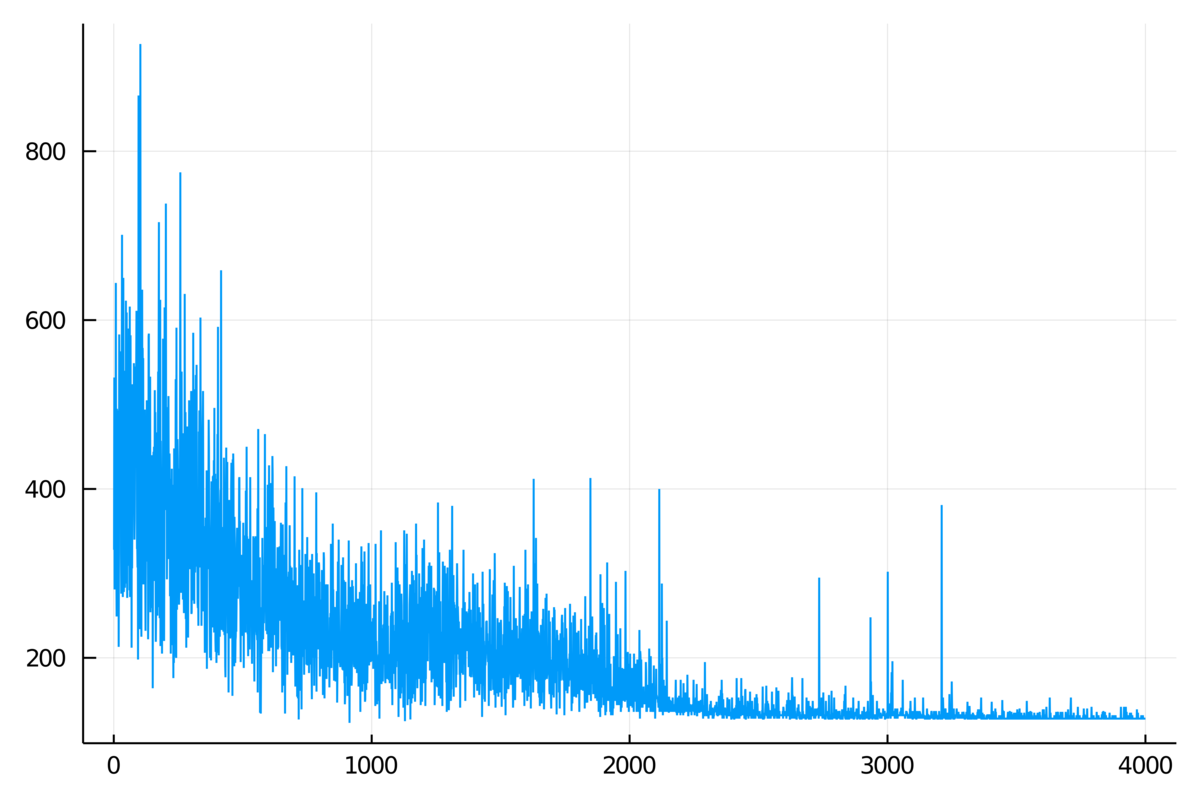
\includegraphics[width=\textwidth]{rews_En3_4k_3layer.png}
    \caption{3 layers trained on a single ideal.}
    \label{subfig:three_layers}
  \end{subfigure}
  \hfill
  \begin{subfigure}[b]{0.49\textwidth}
    \centering
    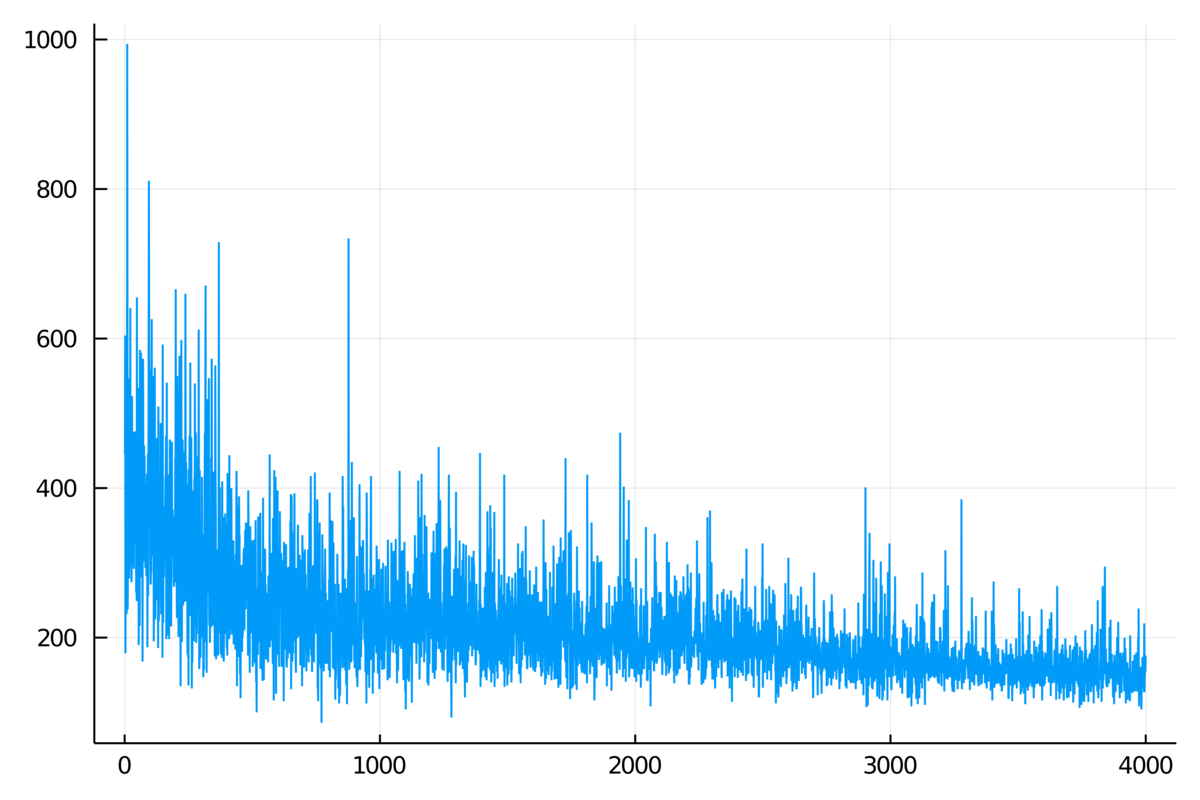
\includegraphics[width=\textwidth]{rews_En3_4k_2layer.png}
    \caption{2 layers trained on a single ideal.}
  \end{subfigure}
  \caption{Comparison of model sizes when training on a single ideal.}
  \label{fig:single_ideal}
\end{figure}


Going up the full training set, we trained the model on dynamically generated ideals.  The performance turned out to match the degree strategy but did not exceed it significantly. We theorize this is because we did not implement GAE (see section \ref{ssec:AE}) but instead went with baseline normalization. The results can be seen in table \ref{tab:eval}

\begin{table}
  \centering
  \begin{tabular}{l|rrr}
    Strategy & Random & Degree & Agent \\
    Score    &  398.7 &  219.6 & 206.4
  \end{tabular}
  \caption{Evaluation of the final model trained on random ideals generated by 4 polynomials of degree less than 10 over three variables. Result is average of 1000 random ideals.}
  \label{tab:eval}
\end{table}

The model was trained on 24000 ideals using an ADAM optimizer with a learning rate of $10^{-4}$. We tried finetuning the model by running it for another 8000 iterations with learning rate $10^{-5}$ but this did not improve performance. The training process\footnote{A moving average is very important here. Since the variance of rewards is high, the plot is dense without the averaging and you can't see any improvement.} can be seen in figure \ref{fig:convergence}.

\begin{figure}[h!]
  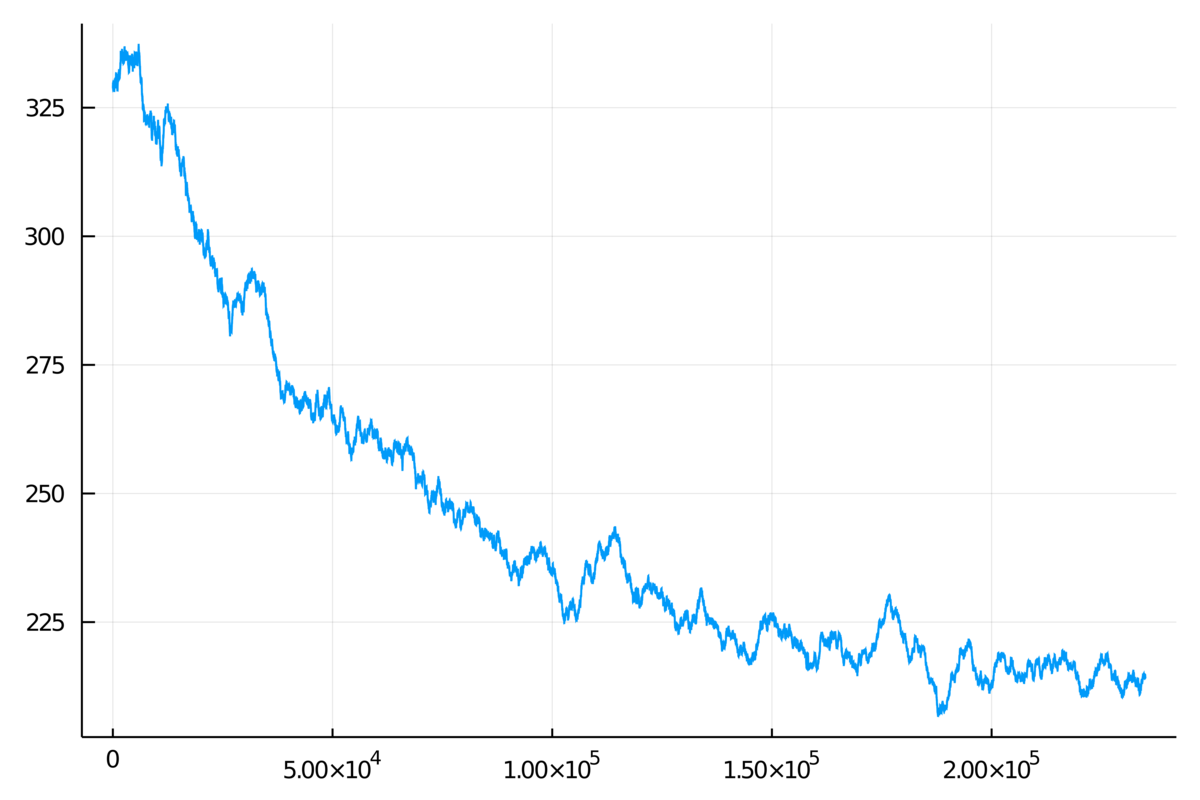
\includegraphics[width=0.9\textwidth]{full_24k_En4_2layer.png}
  \caption{Convergence of the neural network. The graph shows a running average of polynomial additions for each network update with window size 1000.}
  \label{fig:convergence}
\end{figure}

After this we tried the more traditional technique using Q-learning. Performance here did not stabilize, but reached 290 additions, which is not an improvement over standard strategies and increasing the size of the network didn't improve it. This might be due to the unstable nature of rewards; selecting any given pair can lead to wildly different rewards in different contexts, making it difficult to estimate the expected reward.

We could try the normalize rewards similarly to the policy gradient method, but the point of using Q-learning is the simpler implementation. We see no reason to expect performance improvements over policy gradient and using advanced normalization would defeat the simplicity. We have therefore not explored this further.

\subsection{Additional features}
A common way to improve a neural networks performance is to add more information, called features, to the input. This presents the network with information that it doesn't have to compute itself, so it can possibly learn more high-level patterns.

Peifer introduced a novel strategy of selecting the pair whose S-polynomial have the least degree. To help the network I added a number of extra features to the input vector: the encoded pair, then their S-polynomial, then the total degree of the two polynomials and then the degree of their S-polynomial. Somewhat surprisingly, this didn't improve performance. The reason is probably the high variance of rewards and further suggests the importance of GAE. This also suggests that the way to make progress in this domain is novel ways to reduce the variance of rewards.

\section{Technological choices and demo}
We chose to write the code for this experiment in Julia \cite{julia} using the Flux \cite{Flux.jl} framework for deep learning and building the ReinforcementLearning.jl \cite{ReinforcementLearning.jl} project as a skeleton for reinforcement learning.

Writing the program in Julia had two advantages: we could keep all the code in a single language and we improved running time significantly over the implementation by \cite{peifer}.

Taking a look at \url{https://github.com/dylanpeifer/deepgroebner} we see that $\sim 25\%$ of the project is written in C++. This is an implementation of the Buchberger algorithm and code supporting that and it's necessary to keep the code fast. However, a TensorFlow model is built in Python and they must use Python code to bridge between TensorFlow and the custom Buchberger code, even though both are written in C++. This incurs a cost, both on the programmer who needs to learn two languages, and on the runtime. Converting between Python and C++ is not free and since this exchange needs to happen at each selection, taking approximately 100 selections to produce a Gröbner basis, this cross-over happens about 8.000.000 times during a training run.

By keeping everything in Julia, which is a very fast language, we only need to learn a single language, and we prevent the overhead. In practice, this means that we can train the same models as they did in similar timeframes but on an Intel i5 CPU instead of a c5n.xlarge AWS instance even with a naive implementation.


\section{Hitchhikers guide to the code}
The code for this project can be found at \url{https://github.com/0708andreas/Deepgroebner.jl} and is mainly structured into three files.

\begin{enumerate}
  \item groebner.jl holds general code for working with multinomials and computing Gröbner bases. This is the code you could also find in an advanced computer algebra system.

  \item GroebnerEnv.jl holds the code for the environment for the agent to interact with.

  \item model.jl holds the setup code to create a new agent and train it.
    
\end{enumerate}

\subsection{groebner.jl}

We start by defining a structure to hold a single term. A term is represented as a coefficient and an exponent vector:
\begin{minted}[breaklines, escapeinside=||, mathescape=true, linenos, numbersep=3pt, gobble=2, frame=lines, fontsize=\small, framesep=2mm]{julia}
 struct term{N}
    l :: GFElem{Int64}    # coefficient
    a :: NTuple{N, Int64} # exponent
end
\end{minted}

Then a multinomial is simply a list of terms. This lets us express several constructions very consicely, for example multiplication:
\begin{minted}[breaklines, escapeinside=||, mathescape=true, linenos, numbersep=3pt, gobble=2, frame=lines, fontsize=\small, framesep=2mm]{julia}
(*)(t :: term, r :: term) = term(t.l * r.l, t.a .+ r.a)
(*)(t :: term, f ) = Ref(t) .* f
\end{minted}

Especially computing the S-polynomial is almost a direct translation of the mathematical definition.
\begin{minted}[breaklines, escapeinside=||, mathescape=true, linenos, numbersep=3pt, gobble=2, frame=lines, fontsize=\small, framesep=2mm]{julia}
S(f, g) = let gamma = lcm(LT(f), LT(g))
    minus((gamma/LT(f))*f, (gamma/LT(g))*g)
end
\end{minted}

This file also houses the multinomial division algorithm (here called \mintinline{julia}{mdiv} instead of \mintinline{julia}{reduce} as reduce has another meaning in Julia), a full implementation of Buchberger's algorithm, code to perform Gebauer\&Möller reduction and a simple implementation of Buchberger's S-criterion:

\begin{minted}[breaklines, escapeinside=||, mathescape=true, linenos, numbersep=3pt, gobble=2, frame=lines, fontsize=\small, framesep=2mm]{julia}
function is_groebner_basis(G)
    return all([mdiv(S(G[i], G[j]), G) == [] for i in 1:length(G) for j in i:length(G)])
end
\end{minted}


\subsection{GroebnerEnv.jl}
In GroebnerEnv.jl we find the \mintinline{julia}{GroebnerEnv} structure. It is a subtype of an \mintinline{julia}{AbstractEnv}, which is defined in the package ReinforcementLearning.jl. We make good use of this package to provide the structure of reinforcement learning.

The \mintinline{julia}{GroebnerEnv} structure holds a parameters field containing the number of variables in the multinomials, the maximum degree of binomials and how many generators to use for each ideal. It also holds the not-yet-finished Gröbner basis $G$, the list of pairs to reduce $P$ as well as the reward given for the last action, whether we've completed the Gröbner basis or not, how many selections we've performed and a random number generator.

\begin{minted}[breaklines, escapeinside=||, mathescape=true, linenos, numbersep=3pt, gobble=2, frame=lines, fontsize=\small, framesep=2mm]{julia}
mutable struct GroebnerEnv{N, R<:AbstractRNG} <: AbstractEnv
    params::GroebnerEnvParams
    G::Array{Array{term{N}, 1}, 1}
    P::Vector{NTuple{2, Array{term{N}, 1}}}
    reward::Int
    done::Bool
    t::Int
    rng::R
end
\end{minted}

The interaction with the environment is as follows: the environment is initialized with a call to \mintinline{julia}{RLBase.reset!(env)}. Then the result of \mintinline{julia}{RLBase.state(env)} is given to the agent, which picks a number $a$ between 1 and \mintinline{julia}{length(P)}. Then we call \mintinline{julia}{env(a}) which selects the \mintinline{julia}{a}'th pair, reduces it, adds the result to the Gröbner basis, adds new pairs to $P$ and updates \mintinline{julia}{env.reward}. This process is repeated until \mintinline{julia}{env.done} is set to true.

This file also holds a function \mintinline{julia}{eval_model} which is used to evaluate the agents performance.

\subsection{model.jl}
The model.jl file holds the code for both a Q-learner and a policy gradient learner. If we focus on the policy gradient learner, since that's one we got to work well, it's a structure holdning an approximator (a neural network) and baseline network as well as the decay factor $\gamma$ and some other parameters.

The function for interacting with the environment looks like this:

\begin{minted}[breaklines, mathescape=true, linenos, numbersep=3pt, gobble=0, frame=lines, fontsize=\small, framesep=2mm]{julia}
function (pi::VPGPolicy)(env::AbstractEnv)
    to_dev(x) = send_to_device(device(pi.approximator), x)

    logits = env |> state |> to_dev |> pi.approximator

    dist = softmax(logits; dims=2)
    w = Weights(dropdims(dist; dims=1))
    action = sample(pi.rng, 1:length(w), w)

    action
end
\end{minted}

It applies the approximator to \mintinline{julia}{state(env)}, takes \mintinline{julia}{softmax} on the resulting vector and uses that as a probability distribution from which to sample the action.

Next, we have an update function, which updates the agent after each episode. Condensed, the looks like this.

\begin{minted}[breaklines, mathescape=true, linenos, numbersep=3pt, gobble=0, frame=lines, fontsize=\small, framesep=2mm]{julia}
function RLBase.update!(
    pi::VPGPolicy,
    traj::ElasticSARTTrajectory,
    env::AbstractEnv,
    ::PostEpisodeStage,
)
    states = traj[:state]
    actions = traj[:action] |> Array # need to convert ElasticArray to Array, or code will fail on gpu
    gains = traj[:reward] |> x -> discount_rewards(x, pi.gamma)

    for idx in Iterators.partition(shuffle(1:length(traj[:terminal])), pi.batch_size)
        S = select_last_dim(states, idx)
        A = actions[idx]
        G = gains[idx] |> x -> Flux.unsqueeze(x, 1)

        gs = gradient(Flux.params(pi.baseline)) do # update baseline
            d = gains[idx] .- [maximum(pi.baseline(s)) for s in S]
            loss = mean(d .^ 2) # MSE
            Zygote.ignore() do
                pi.baseline_loss = loss
            end
            loss
        end
        RLBase.update!(pi.baseline, gs)

        gs = gradient(Flux.params(model)) do
            log_prob = [logsoftmax(model(s); dims=2) for s in S]
            log_prob_a = [log_prob[i][A[i]] for i in 1:length(A)]
            loss = -mean(log_prob_a .* d)

            Zygote.ignore() do
                pi.loss = loss
            end
            loss
        end
        RLBase.update!(model, gs)
    end
end
\end{minted}

The code uses julias broadcast operators, so \mintinline{julia}{a .* b} is the entry-wise product of two vectors $a$ and $b$. Similarly \mintinline{julia}{d .^ 2} squares each entry of the vector $d$.

Finally, we set up the experiment:
\begin{minted}[breaklines, mathescape=true, linenos, numbersep=3pt, gobble=0, frame=lines, fontsize=\small, framesep=2mm]{julia}
function pg_experiment(  params :: GroebnerEnvParams,
                         episodes :: Int,
                         learn_rate = 10^-3,
                         gamma = 0.99f0,
                         seed = 123;
                         env = nothing)

    rng = StableRNG(seed)

    n = params.nvars
    d = params.maxdeg
    s = params.npols

    if env == nothing
        env = rand_env(params)
    end

    agent = Agent(
        policy = VPGPolicy(
            approximator = NeuralNetworkApproximator(
                model = Chain(
                    Dense(n*4, 64, relu; initW = glorot_uniform(rng)),
                    Dense(64, 1; initW = glorot_uniform(rng))
                ),
                optimizer = ADAM(learn_rate),

            ) |> cpu,
            baseline = NeuralNetworkApproximator(
                model = Chain(
                    Dense(n*4, 64, relu; initW = glorot_uniform(rng)),
                    Dense(64, 1; initW = glorot_uniform(rng)),
                ),
                optimizer = ADAM(learn_rate),
            ) |> cpu,
            gamma = gamma,
            rng = rng,
        ),
        trajectory = ElasticSARTTrajectory(state = Vector{Array{Int, 2}} => (),
                                            reward = Int => ()),
    )

    stop_condition = StopAfterEpisode(episodes)

    total_reward_per_episode = TotalRewardPerEpisode()
    time_per_step = TimePerStep()
    hook = ComposedHook(
        total_reward_per_episode,
        time_per_step,
    )

    description = "# Make Gröbner bases with Policy Gradients"

    Experiment(agent, env, stop_condition, hook, description)
end
\end{minted}
and this experiment can be run in an interactive shell like this:

\begin{minted}[breaklines, escapeinside=||, mathescape=true, linenos, numbersep=3pt, gobble=0, frame=lines, fontsize=\small, framesep=2mm]{julia}
  using Deepgroebner
  params = GroebnerEnvParams(3, 10, 4, nothing)
  e = pg_experiment(params, 120_000, 10^-4)
  run(e)

  eval_model(m_pg.env, strat_rand)
  eval_model(m_pg.env, strat_degree)
  eval_model(m_pg.env, m_pg.policy)
\end{minted}
which also uses the \mintinline{julia}{eval_model} function to compare the trained model against two standard strategies.


\printbibliography

\appendix
\section{Code}
The code described and used in this report can be found at \url{https://gitlab.au.dk/au612120/Deepgroebner.jl}. The commit used is \\ 018527d0e32f40405ceaccc9ffdba8412f40deb0, permalink: \url{https://gitlab.au.dk/au612120/Deepgroebner.jl/-/tree/018527d0e32f40405ceaccc9ffdba8412f40deb0}

\section{Definitions and elementary properties}
Use this section as a reference for elementary algebra terms.

\begin{definition}[Ring, commutative ring]
  A \emph{ring} $R$ is a set with two binary operations $+, \times$ and a unary operation $-$ satisfying:
  
  \begin{enumerate}
    \item $\forall x, y \in R: x + y = y + x$
    \item $\forall x, y, z \in R: x + (y + z) = (x + y) + z$
    \item $\exists 0 \in R \forall x \in R : 0 + x = x + 0 = x$
    \item $\forall x \in R: -a + a = a + (-a) = 0$
    \item $\forall x, y, a \in R: x \times (y \times z) = (x \times y) \times z$
    \item $\exists 1 \in R \forall x \in R : 1 \times x = x \times 1 = x$
    \item $\forall x, y, z \in R: x \times (y + z) = (x \times y) + (x \times z)$
    \item $\forall x, y, z \in R: (x + y) \times z = (x \times z) + (y \times z)$
  \end{enumerate}

  (1)-(4) means that $(R, +, 0)$ is a commutative group, (5)-(6) means that $(R, \times, 1)$ is a monoid and (7)-(8) says that multiplication distributes over addition.

  A \emph{commutative ring} also satisfies $\forall x, y \in R: x \times y = y \times x$.
\end{definition}

Note that a field is also a commutative ring and that given a given a commutative ring $R$, the set of polynomials with coefficients in $R$ form a commutative ring.

\begin{definition}[Ideal]
  Given a commutative ring $R$ an \emph{ideal} in $R$ is a set $I \subseteq R$ such that
  \begin{itemize}
      \item $\forall x, y \in I: x + y \in I$
      \item $\forall x \in R, y \in I: x \times y \in I$
  \end{itemize}
\end{definition}

A simple example of an ideal in the ring of integers is sets of the form $[n] = \{nx \mid x \in \m Z\}$. In general, given a finite set of elements $X = \{x_{1}, x_{2}, \dots, x_{t}\} \subseteq R$ we can generate an ideal from these elements: \[\tuple X = \left\{\sum_{i = 1}^{t} a_{i} x_{i} \mid a_{i} \in R\right\}.\] This is the set of linear combinations of the elements from $X$.

\begin{definition}[Generating set]
  A \emph{generating set} for an ideal $I$ is a finite set of elements $X \subseteq I$ such that $I = \tuple X$
\end{definition}

The ring of polynomials over a field have the property that every ideal has a generating set.

\end{document}
